% !TEX program = xelatex
% 컴파일: xelatex whitepaper.tex (kotex + Apple SD Gothic Neo)
\documentclass[11pt]{article}

\usepackage{kotex}
\setmainhangulfont{Apple SD Gothic Neo}
\setsanshangulfont{Apple SD Gothic Neo}

\usepackage{amsmath}
\usepackage{amssymb}
\usepackage{graphicx}
\usepackage{booktabs}
\usepackage{xcolor}
\usepackage{titlesec}
\usepackage{caption}
\usepackage{enumitem}
\usepackage{fancyhdr}
\usepackage[a4paper, top=2.6cm, bottom=2.6cm, left=2.8cm, right=2.8cm]{geometry}
\usepackage{hyperref}

\graphicspath{{../figures/}}

% ----- 브랜드 색상 -----
\definecolor{brand}{RGB}{140,22,22}      % 딥 레드 (컨설팅 백서 톤)
\definecolor{ink}{RGB}{40,40,40}
\definecolor{rulegray}{RGB}{200,200,200}

\hypersetup{
  colorlinks=true, linkcolor=brand, urlcolor=brand, citecolor=brand,
  pdftitle={누구에게 어떤 프로모션을 제공해야 할까},
  pdfauthor={Haechang Cho}
}

% ----- 섹션 스타일 -----
\titleformat{\section}{\sffamily\Large\bfseries\color{brand}}{\thesection.}{0.5em}{}
\titleformat{\subsection}{\sffamily\large\bfseries\color{ink}}{\thesubsection}{0.5em}{}
\titlespacing*{\section}{0pt}{1.6em}{0.7em}

% ----- 캡션 스타일 -----
\captionsetup{font=small, labelfont={bf,color=brand}, labelsep=period, skip=6pt}

% ----- 머리말/꼬리말 -----
\pagestyle{fancy}
\fancyhf{}
\renewcommand{\headrulewidth}{0pt}
\renewcommand{\footrulewidth}{0.4pt}
\renewcommand{\footrule}{\hbox to\headwidth{\color{rulegray}\leaders\hrule height \footrulewidth\hfill}}
\fancyfoot[L]{\footnotesize\color{brand} 누구에게 어떤 프로모션을 제공해야 할까 · 정책학습 기반 타겟팅}
\fancyfoot[R]{\footnotesize\color{brand}\thepage}

\setlength{\parskip}{0.6em}
\setlength{\parindent}{0pt}
\renewcommand{\arraystretch}{1.25}

% 핵심 수치 강조용
\newcommand{\kpi}[1]{{\color{brand}\bfseries #1}}

\begin{document}

% =================================================== 표지
\thispagestyle{empty}
\vspace*{1.2cm}
{\sffamily\bfseries\color{brand}\large CAUSAL INFERENCE PORTFOLIO}
\vskip 2pt
{\color{rulegray}\hrule height 1.2pt}

\vspace{4.5cm}
{\sffamily\bfseries\fontsize{30}{36}\selectfont 누구에게 어떤 프로모션을\\[4pt] 제공해야 할까?\par}
\vspace{0.8cm}
{\sffamily\Large\color{ink} 예산 제약 하의 정책학습(Policy Learning) 기반 프로모션 타겟팅\par}

\vspace{3.2cm}
{\sffamily\large\bfseries\color{brand} 데이터 분석 포트폴리오\par}

\vfill
{\footnotesize\color{ink}
\textbf{Haechang Cho} \quad
GitHub: \href{https://github.com/Funbucket}{github.com/Funbucket} \quad
LinkedIn: \href{https://www.linkedin.com/in/hae-chang-cho/}{hae-chang-cho}\par
\vskip 4pt
관찰 데이터 · 다중 처치 · Doubly Robust(AIPW) · econml DRLearner/DRPolicyTree/DRPolicyForest
}
\newpage

% =================================================== 요약
\section*{\sffamily\color{brand} 요약 (Executive Summary)}
\addcontentsline{toc}{section}{요약}

\textbf{문제.} 한 소프트웨어 회사는 고객에게 \emph{기술지원}과 \emph{할인} 두 가지 프로모션을 제공할 수 있다(두 개입의 조합으로 총 네 가지 처치). 예산은 제한되어 있고, 프로모션 효과는 고객마다 다르다. 따라서 핵심 질문은 다음과 같다: \textbf{``제한된 예산 안에서 누구에게 어떤 프로모션을 제공해야 전체 순이익이 가장 커질까?''}

\textbf{접근.} 약 2{,}000명의 \textbf{관찰 데이터}에 정책학습(policy learning)을 적용했다. (1)~처치 효과의 이질성을 진단하고, (2)~관찰 데이터의 인과 식별 가정을 점검한 뒤, (3)~세 가지 정책(DRLearner plug-in · DRPolicyTree · DRPolicyForest)을 학습하고, (4)~학습/평가 데이터를 분리해 \textbf{AIPW(doubly robust) score}로 정책 가치를 비교했으며, (5)~예산 제약 하의 효율은 \textbf{비용 곡선(cost curve)}으로 평가했다.

\textbf{핵심 결과.}

\begin{table}[h]
\centering
\small
\begin{tabular}{lrr}
\toprule
정책 & 1인당 평균 순이익 & 무처치 대비 \\
\midrule
무처치 (all none) & \$7{,}249 & --- \\
최선의 단일 처치 (전원 기술지원) & \$10{,}527 & +45\% \\
\textbf{고객별 타겟팅 (DRLearner plug-in)} & \kpi{\$11{,}798} & \kpi{+63\%} \\
\bottomrule
\end{tabular}
\end{table}

\begin{itemize}[leftmargin=1.4em, itemsep=2pt]
  \item 고객별 타겟팅 정책은 가장 좋은 \textbf{단일 처치 정책보다 약 12\%}, 무처치 대비 약 63\% 높은 순이익을 냈다.
  \item 처치 배정을 좌우한 핵심 요인은 \textbf{직원 수(42\%)와 고객 규모(38\%)}였다. 규모가 큰 고객에게는 \emph{기술지원+할인}을, 그 외 고객에게는 주로 \emph{기술지원}을 배정했다.
  \item \textbf{예산 수준에 따라 최적 정책이 달랐다.} 소액 예산에서는 평균 비용이 낮은 \emph{전원 기술지원}이 가장 효율적이지만, 예산이 1인당 \$4{,}000\,$\sim$\,6{,}000 수준으로 커지면 학습 정책이 더 높은 순이익을 냈다.
\end{itemize}

\textbf{권고.} 모두에게 동일한 프로모션을 적용하기보다, \textbf{고객 규모·직원 수에 기반한 타겟팅 규칙}을 적용할 것을 권고한다. 성능을 최우선한다면 plug-in/forest 정책을, 이해관계자 설명과 운영 안정성이 중요하다면 약간의 성능을 양보하더라도 해석 가능한 \textbf{depth=2 의사결정 트리 정책}을 권장한다.

\newpage

% =================================================== 1. 비즈니스 문제
\section{비즈니스 문제}

인과추론의 많은 문제는 평균 처치 효과(ATE)에 집중한다. ``프로모션을 진행할 것인가, 하지 않을 것인가?''라는 질문은 \emph{모든} 고객에게 동일한 프로모션을 제공하는 정책과 아무에게도 제공하지 않는 정책을 비교하는 문제다.

하지만 예산이 제한되어 있고 그 안에서 최대 효과를 내야 한다면 이야기가 달라진다. 프로모션 효과가 고객마다 다르다면, 모두에게 동일하게 제공하는 전략이 최선이 아닐 수 있다.

\begin{itemize}[leftmargin=1.4em, itemsep=2pt]
  \item 마케팅 유무와 상관없이 어차피 구매하거나(\emph{always-converters}), 반대로 아무리 혜택을 줘도 사지 않을 고객(\emph{lost causes})에게 불필요한 예산을 낭비하게 된다.
  \item 마케팅에 부정적으로 반응하는 고객(\emph{sleeping dogs}) 때문에 오히려 손실이 발생하며,
  \item 정작 효과가 클 고객(\emph{high-responders})을 우선순위에 두지 못해 잠재 매출을 놓친다.
\end{itemize}

따라서 이 분석이 답하려는 질문은 \emph{``어떤 고객을 대상으로 해야 순이익이 가장 커질까?''}이다. 가능한 처치 규칙들을 탐색해 전체 평균 순수익을 근사적으로 최대화하는 문제, 즉 \textbf{``누구를 처치해야 하는가?''}에 답하는 문제를 \textbf{정책학습(policy learning)}이라고 부른다.

이 백서는 다음 다섯 가지 질문으로 구성된다.

\begin{description}[leftmargin=2.4em, itemsep=2pt]
  \item[Q1.] 프로모션 효과는 정말 고객마다 다른가? (이질성 진단)
  \item[Q2.] 관찰 데이터로 인과 효과를 신뢰할 수 있는가? (식별 가정)
  \item[Q3.] 누구에게 무엇을 배정해야 하는가? (정책학습)
  \item[Q4.] 학습한 정책이 정말 더 나은가? (정책 평가)
  \item[Q5.] 예산이 제한되면 어떤 정책이 유리한가? (예산 제약)
\end{description}

% =================================================== 2. 데이터
\section{데이터와 처치 정의}

무작위 실험(RCT)이 가장 이상적이지만, 실제 비즈니스 환경에서는 비용 문제, 영업 전략, 대형 고객을 놓칠 위험 등으로 무작위 실험을 수행하기 어렵다. 따라서 이번 데이터는 무작위 실험 데이터가 아닌 \textbf{관찰 데이터}이며, 약 2{,}000명의 고객 정보로 구성된다(고객 특성 8종, 개입 2종, 결과 1종).

\texttt{Tech Support}와 \texttt{Discount}는 모두 개입이므로, 이를 조합해 네 가지 처치로 정의한다($A_i \in \{0,1,2,3\}$).

\begin{table}[h]
\centering
\small
\caption{네 가지 처치 정의}
\begin{tabular}{cll}
\toprule
$A_i$ & 이름 & 의미 \\
\midrule
0 & none & 아무 개입도 제공하지 않음 \\
1 & tech\_support\_only & 기술지원만 제공 \\
2 & discount\_only & 할인만 제공 \\
3 & discount\_plus\_support & 기술지원과 할인을 모두 제공 \\
\bottomrule
\end{tabular}
\end{table}

\subsection{비용 설정}

수익 극대화를 위해서는 매출과 함께 \textbf{비용}도 고려해야 한다. 동일한 프로모션이라도 고객 특성에 따라 비용이 달라질 수 있다. 이 데이터에는 실제 비용 정보가 없으므로, 기술지원 비용은 직원 수가 많을수록, 할인 비용은 고객 규모가 클수록 증가하도록 \textbf{시뮬레이션}한다. 비용이 항상 양수이고 일부 고객에서 큰 비용이 발생하는 분포를 반영하기 위해 로그정규분포를 사용한다.

\[
C_i(\text{tech}) \sim \text{LogNormal}(\log C_{\text{tech}} + 0.5\,\tilde{e}_i,\ 0.3), \qquad
C_i(\text{disc}) \sim \text{LogNormal}(\log C_{\text{disc}} + 0.4\,\tilde{s}_i,\ 0.3)
\]

여기서 $\tilde{e}_i$는 표준화된 직원 수, $\tilde{s}_i$는 표준화된 회사 규모다. 고객별 비용을 반영한 최종 \textbf{순이익(net outcome)}은 $Y_i^{net} = Y_i - C_i(A_i)$로 정의한다. 이렇게 하면 이후 AIPW score가 순이익 기준으로 계산되어, 비용을 고려한 정책 최적화와 평가가 가능해진다. 정책 학습과 평가는 train/test를 50:50으로 분리해(각 1{,}000명) 과대추정을 방지한다.

% =================================================== Q1
\section{Q1. 프로모션 효과는 정말 고객마다 다른가?}

타겟팅이 의미가 있으려면 먼저 \textbf{처치 효과가 고객마다 다르다}는 신호가 있어야 한다. 처치별 표본은 23\,$\sim$\,27\%로 고르게 분포해(표~\ref{tab:summary}) 비교에 안정적이다. 한편 처치별 평균 매출은 무처치 6{,}586에서 기술지원+할인 26{,}784까지 크게 다르다.

\begin{table}[h]
\centering
\small
\caption{처치별 표본 수·평균 매출·평균 비용·평균 순이익}
\label{tab:summary}
\begin{tabular}{lrrrr}
\toprule
처치 & 표본 수 & 평균 매출 & 평균 비용 & 평균 순이익 \\
\midrule
none & 517 & 6{,}586 & 0 & 6{,}586 \\
tech\_support\_only & 462 & 15{,}104 & 5{,}038 & 10{,}066 \\
discount\_only & 477 & 12{,}248 & 5{,}182 & 7{,}066 \\
discount\_plus\_support & 544 & 26{,}784 & 12{,}665 & 14{,}119 \\
\bottomrule
\end{tabular}
\end{table}

그러나 이 평균 차이를 그대로 처치 효과로 해석하면 안 된다. 그림~\ref{fig:cov}에서 보듯 처치 그룹별 고객 특성이 다르고(특히 \texttt{Size}, \texttt{IT Spend}), 규모가 큰 고객일수록 더 강한 개입을 받는 경향이 있다. 즉 매출 차이에는 고객 특성의 영향과 실제 처치 효과가 함께 섞여 있다(그림~\ref{fig:rev}).

\begin{figure}[h]
\centering
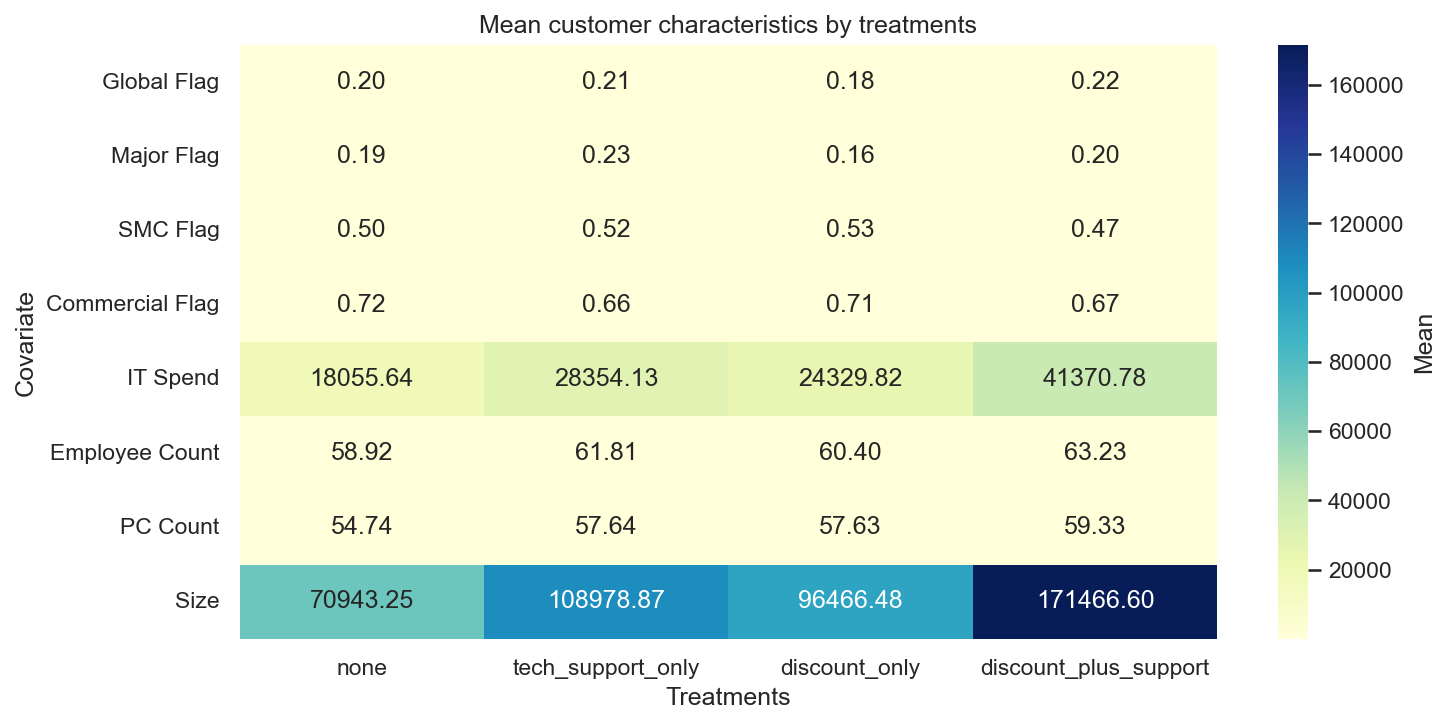
\includegraphics[width=0.82\textwidth]{fig02_covariate_means.png}
\caption{처치별 고객 특성 평균. \texttt{Size}, \texttt{IT Spend}가 처치 그룹마다 다르게 나타나며, 처치 배정이 고객 특성과 얽혀 있음을 보여준다.}
\label{fig:cov}
\end{figure}

\begin{figure}[h]
\centering
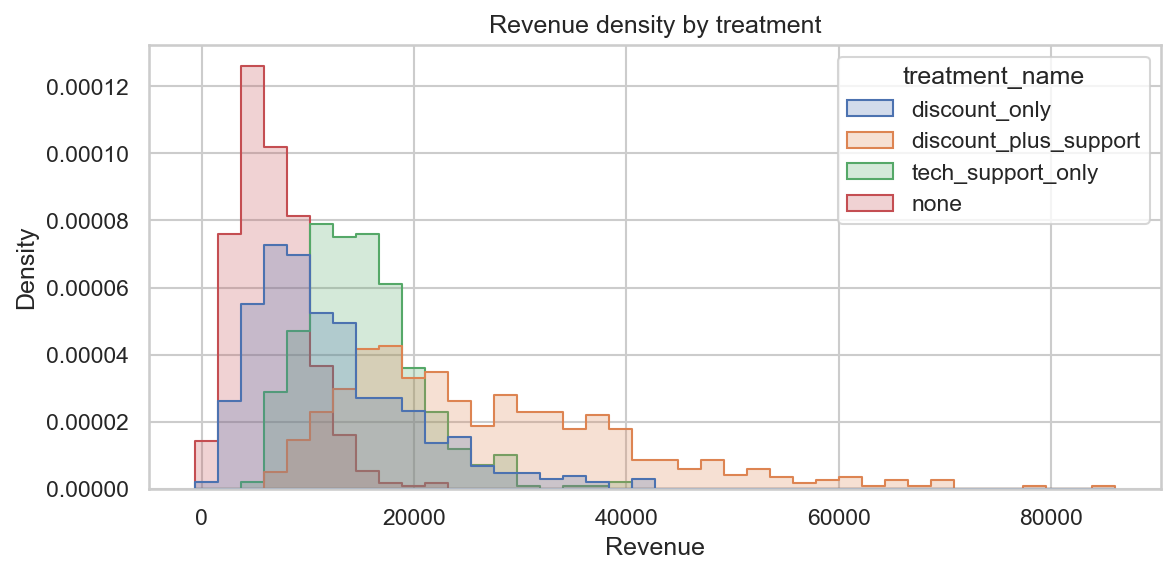
\includegraphics[width=0.72\textwidth]{fig03_revenue_dist.png}
\caption{처치별 Revenue 분포. 규모·분산·이상치가 처치마다 다르다.}
\label{fig:rev}
\end{figure}

\textbf{Q1 요약.} 처치 그룹 간 고객 특성과 결과 분포가 뚜렷이 다르다. 이는 (a)~처치 효과가 고객마다 다를 가능성과 (b)~처치 배정이 고객 특성에 의해 교란되어 있음을 동시에 시사한다. 따라서 단순 평균 비교가 아니라 교란을 보정하는 인과적 접근이 필요하다.

% =================================================== Q2
\section{Q2. 관찰 데이터로 인과 효과를 신뢰할 수 있는가?}

관찰 데이터에서 AIPW 추정이 인과적으로 유효하려면 두 가지 가정이 필요하다.

\textbf{1. Unconfoundedness (비교란성).}\quad
$\{Y_i(0), Y_i(1), Y_i(2), Y_i(3)\} \perp A_i \mid X_i$. 관측된 공변량 $X_i$를 조건부로 했을 때 처치 배정이 잠재 결과와 독립이어야 한다. 즉, 고객 규모·IT 지출·직원 수 등이 처치 배정을 충분히 설명한다고 가정한다.

\textbf{2. Positivity (양수성).}\quad
$P(A_i = a \mid X_i = x) > 0,\ \forall a,\ \forall x$. 모든 고객 특성 범위에서 각 처치가 어느 정도 관측되어야 한다. 이는 propensity score $e_a(x) = P(A_i = a \mid X_i = x)$를 추정해 직접 확인할 수 있다.

\begin{figure}[h]
\centering
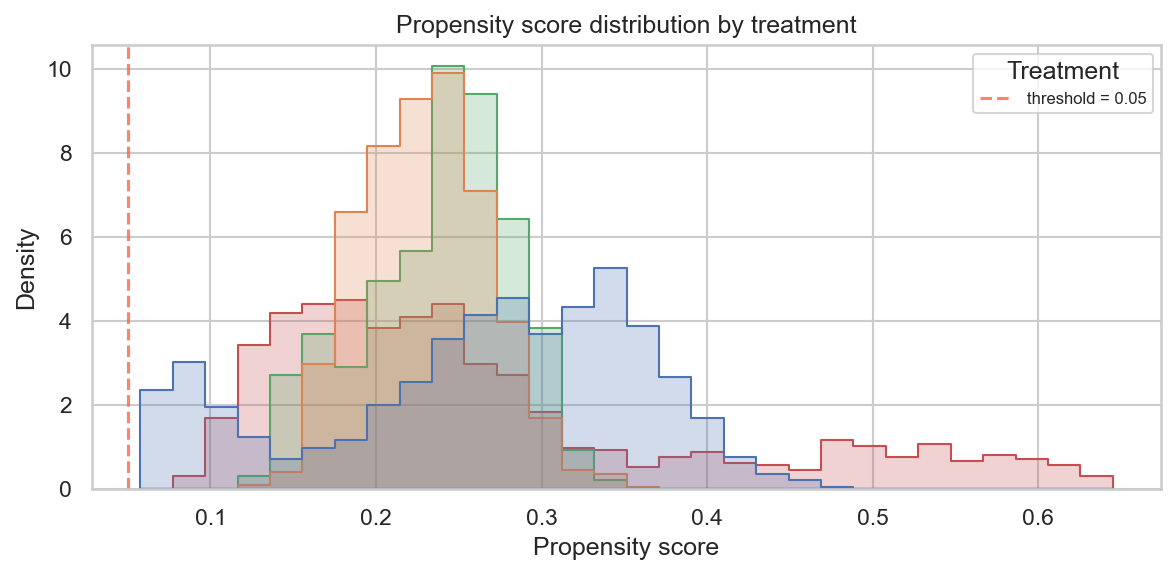
\includegraphics[width=0.72\textwidth]{fig04_propensity.png}
\caption{처치별 propensity score 분포. 네 처치의 분포가 잘 겹치며, $\hat e_a(X_i)$의 최솟값은 약 0.058로 \texttt{0.05} 미만 관측치가 없다.}
\label{fig:prop}
\end{figure}

이 데이터에서 $\hat e_a(X_i)$의 최솟값은 약 \textbf{0.058}이며, \texttt{0.05} 미만 관측치도 없다(그림~\ref{fig:prop}). 즉 극단적으로 작은 propensity score로 일부 관측치에 과도한 가중치가 부여되는 문제는 크지 않다.

\textbf{Q2 요약.} Positivity는 데이터로 확인되어 충족된다. Unconfoundedness는 검정 불가능한 가정이지만, 처치 배정을 설명할 핵심 변수들이 관측되어 있어 합리적인 가정으로 받아들인다. 따라서 이후 분석은 outcome model과 propensity model을 함께 쓰는 \textbf{doubly robust(AIPW)} 추정을 채택한다.

% =================================================== Q3
\section{Q3. 누구에게 무엇을 배정해야 하는가?}

세 가지 정책을 학습해 비교한다.

\begin{itemize}[leftmargin=1.4em, itemsep=2pt]
  \item \textbf{Plug-in Policy (DRLearner):} 고객별 CATE를 추정한 뒤 기대 순이익이 가장 큰 처치를 선택. 유연하지만 CATE 추정 품질에 민감.
  \item \textbf{DRPolicyTree:} AIPW score를 직접 최대화하되 정책을 얕은 의사결정 트리로 제한 $\Rightarrow$ \textbf{해석 가능}.
  \item \textbf{DRPolicyForest:} AIPW score를 직접 최대화하되 forest 사용 $\Rightarrow$ 분산이 작고 안정적이지만 해석은 어려움.
\end{itemize}

\subsection{Plug-in Policy}
\texttt{none}을 baseline으로 두고 \texttt{DRLearner}로 상대효과 $\hat\tau_a(x) = \widehat{\mathbb{E}}[Y^{net}(a) - Y^{net}(0)\mid X=x]$를 추정한 뒤, 고객별로 $[0, \hat\tau_1(x), \hat\tau_2(x), \hat\tau_3(x)]$를 비교해 가장 큰 처치를 선택한다.
\[
\hat\pi_{\text{plugin}}(x) = \arg\max_{a \in \{0,1,2,3\}} \widehat{\mathbb{E}}[Y^{net}(a) - Y^{net}(0)\mid X=x]
\]
이 정책은 약 50\%에게 기술지원, 37\%에게 기술지원+할인, 약 9\%에게 무처치를 배정한다. 기대 순이익이 음수인 일부 고객에게는 처치하지 않는 선택이 나타난다.

\subsection{Policy Tree}
현업에서는 성능뿐 아니라 \textbf{정책의 설명 가능성}도 중요하다. 얕은 의사결정 트리 정책은 (i)~이해관계자 설명, (ii)~공정성 검토, (iii)~운영 안정성 측면에서 유리하다. 이때 정책을 모든 함수가 아니라 제한된 정책 클래스 $\Pi$(얕은 트리) 안에서 탐색한다.
\[
\hat\pi = \arg\max_{\pi \in \Pi} \frac{1}{n}\sum_{i=1}^{n} \widehat\Gamma_{i,\pi(X_i)}
\]

\begin{figure}[h]
\centering
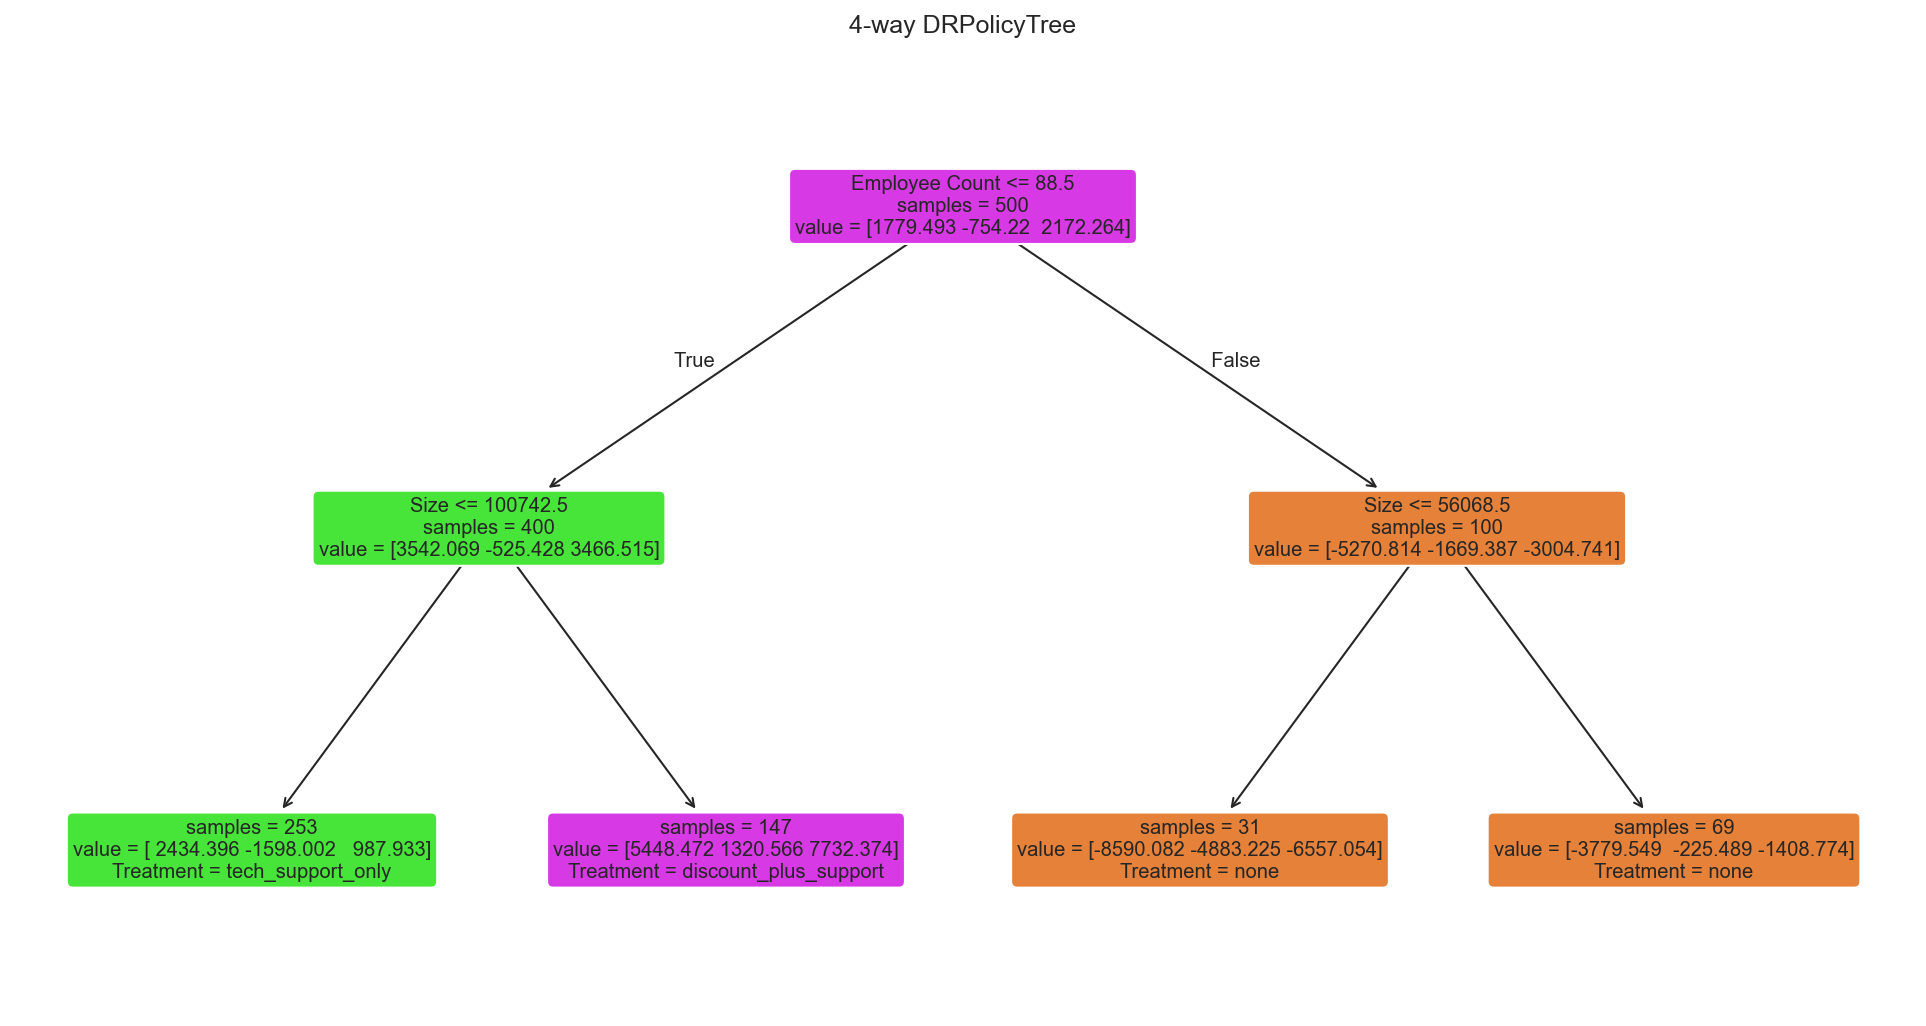
\includegraphics[width=0.95\textwidth]{fig05_policy_tree.png}
\caption{depth=2 DRPolicyTree. 주로 \texttt{Size}를 기준으로 분기한다. 규모가 큰 고객에게는 기술지원+할인을, 그 외에는 주로 기술지원을, 기대 순이익이 낮은 일부(약 20\%)에게는 무처치를 배정한다.}
\label{fig:tree}
\end{figure}

\subsection{Policy Forest와 핵심 변수}
Policy Forest는 단일 트리 대신 여러 트리를 평균해 분산이 작고 복잡한 이질성을 안정적으로 학습한다. 단일 규칙으로 해석하기는 어렵지만, \texttt{feature\_importances\_}로 어떤 특성이 배정을 주도하는지 파악할 수 있다.

\begin{figure}[h]
\centering
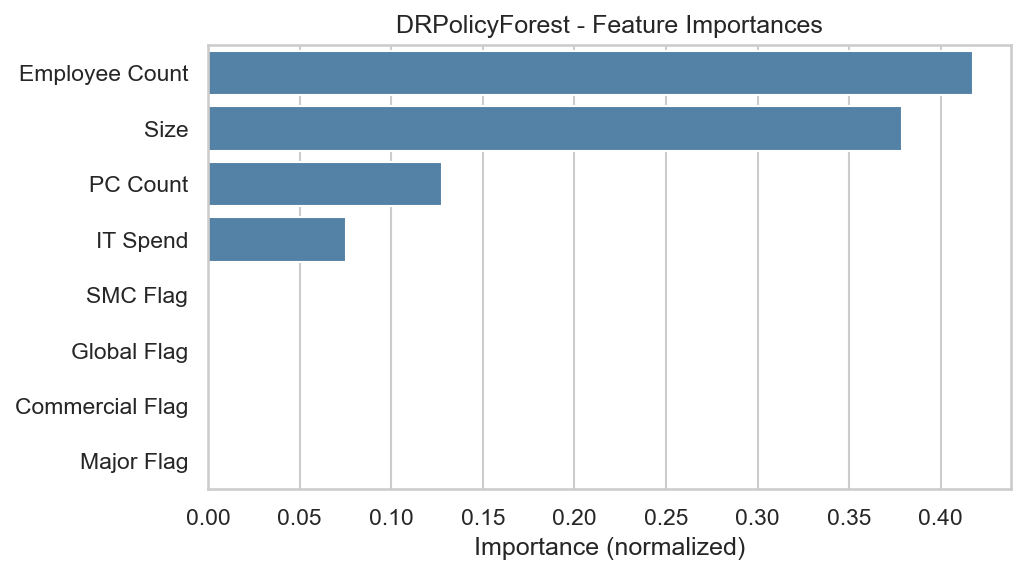
\includegraphics[width=0.7\textwidth]{fig06_feature_importance.png}
\caption{DRPolicyForest 변수 중요도. \texttt{Employee Count}(42\%)와 \texttt{Size}(38\%)가 전체의 약 80\%를 차지한다.}
\label{fig:fi}
\end{figure}

\texttt{Employee Count}(42\%)와 \texttt{Size}(38\%)가 전체 중요도의 약 80\%를 차지하며, \textbf{고객 규모와 직원 수가 처치 배정을 주도}함을 확인할 수 있다(그림~\ref{fig:fi}). 이는 트리 정책이 \texttt{Size}로 분기한 결과(그림~\ref{fig:tree})와도 일치한다.

\textbf{Q3 요약.} 세 정책 모두 ``규모가 큰 고객 $\to$ 기술지원+할인, 그 외 $\to$ 주로 기술지원, 기대 순이익이 낮은 일부 $\to$ 무처치''라는 일관된 배정 패턴을 학습했다.

% =================================================== Q4
\section{Q4. 학습한 정책이 정말 더 나은가?}

학습한 정책들을 동일한 test set의 \textbf{AIPW score} 기준으로, 모든 고객에게 동일 처치를 적용하는 baseline 정책과 함께 비교한다. AIPW(Augmented Inverse Probability Weighting) score는 다음과 같다.
\[
\hat\Gamma_{i,a} = \hat\mu_a(X_i) + \frac{\mathbf{1}[A_i=a]}{\hat e_a(X_i)}\bigl(Y_i^{net} - \hat\mu_a(X_i)\bigr)
\]
여기서 $\hat\mu_a$는 outcome model, $\hat e_a$는 propensity model의 예측이다. 이 구조 덕분에 둘 중 \textbf{하나만 올바르게 추정되어도} 불편성이 유지된다(doubly robust).

\begin{table}[h]
\centering
\small
\caption{정책 가치 비교 (test set AIPW value, 1인당 평균 순이익)}
\label{tab:value}
\begin{tabular}{lrr}
\toprule
정책 & AIPW value & 95\% 신뢰구간 \\
\midrule
\textbf{DRLearner plug-in} & \kpi{11{,}798} & [11{,}270,\ 12{,}326] \\
DRPolicyForest & 11{,}619 & [11{,}095,\ 12{,}143] \\
DRPolicyTree (depth=2) & 11{,}149 & [10{,}701,\ 11{,}596] \\
\midrule
all\_tech\_support\_only & 10{,}527 & [9{,}833,\ 11{,}220] \\
all\_discount\_plus\_support & 10{,}137 & [9{,}439,\ 10{,}834] \\
all\_discount\_only & 7{,}545 & [6{,}994,\ 8{,}097] \\
all\_none & 7{,}249 & [6{,}955,\ 7{,}543] \\
\bottomrule
\end{tabular}
\end{table}

\begin{figure}[h]
\centering
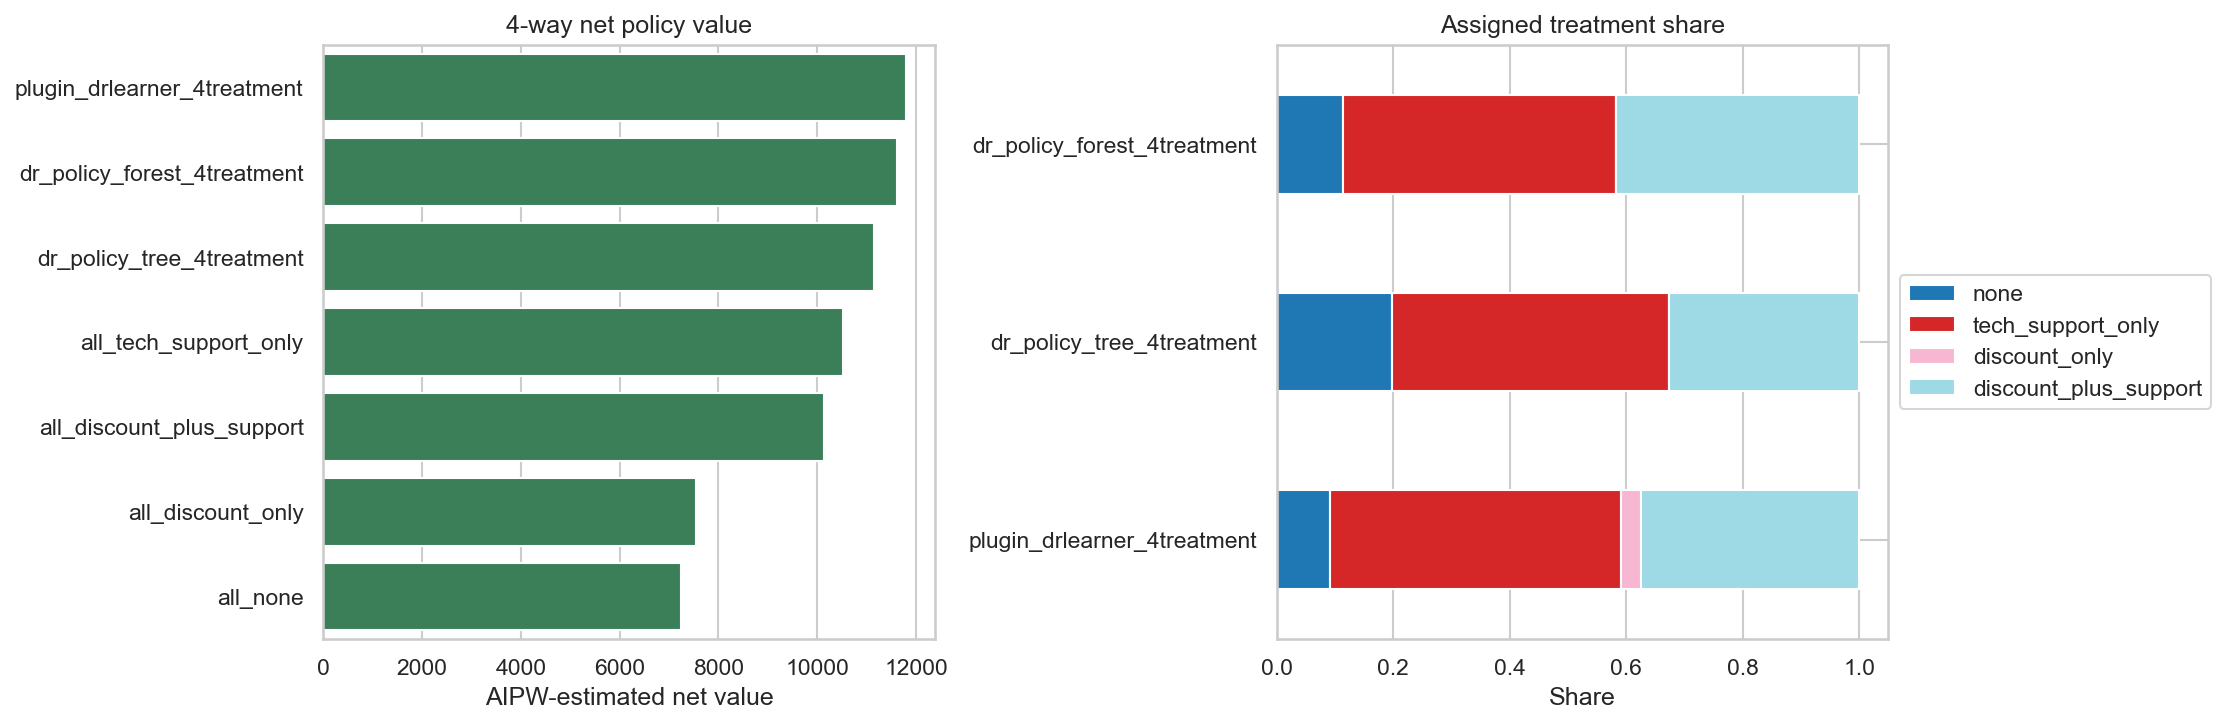
\includegraphics[width=0.95\textwidth]{fig07_policy_value.png}
\caption{(좌) 정책별 AIPW 순가치. 세 학습 정책 모두 단일 처치 정책을 상회한다. (우) 학습 정책의 처치 배정 비중.}
\label{fig:value}
\end{figure}

세 학습 정책 모두 단일 처치 정책보다 높은 가치를 가진다(표~\ref{tab:value}, 그림~\ref{fig:value}). \textbf{고객별 타겟팅이 모두에게 같은 처치를 적용하는 것보다 효과적}이라는 의미다. plug-in과 forest는 신뢰구간이 상당 부분 겹쳐 실질적 차이가 있다고 보기는 어렵다. 트리 정책은 해석 가능성을 유지하는 대신 성능을 일부 양보했다. \texttt{all\_discount\_plus\_support}가 \texttt{all\_tech\_support\_only}보다 낮은 이유는, 할인 비용이 고객 규모에 따라 커지도록 설정해 일부 고객에서 할인의 순수익이 비용을 상쇄하지 못했기 때문이다.

\textbf{Q4 요약.} 세 학습 정책 모두 최선의 단일 처치 정책보다 높은 순이익을 낸다(plug-in 기준 +12\%, 무처치 대비 +63\%). 타겟팅의 가치가 데이터로 확인된다.

% =================================================== Q5
\section{Q5. 예산이 제한되면 어떤 정책이 유리한가?}

지금까지는 전체 AIPW value를 비교했다. 그러나 실제로는 예산이 제한될 수 있다. 같은 예산 안에서 어떤 정책이 더 효율적인지 비교하려면 \textbf{비용 곡선(cost curve)}이 유용하다. 먼저 처치별 고객 기대 비용 $E[C(a)\mid X_i]$를 추정한다(기술지원 \$4{,}892, 할인 \$5{,}454, 둘 다 \$10{,}687, test 평균).

비용 곡선의 x축은 1인당 누적 평균 처치 비용, y축은 1인당 누적 평균 순수익(무처치 대비 증분, 비용 차감 후)이다. 순수익/비용 비율이 높은 고객부터 순서대로 처치하며, $x=B$에서 세로선을 그으면 예산 $B$ 하의 비교가 된다.

\begin{figure}[h]
\centering
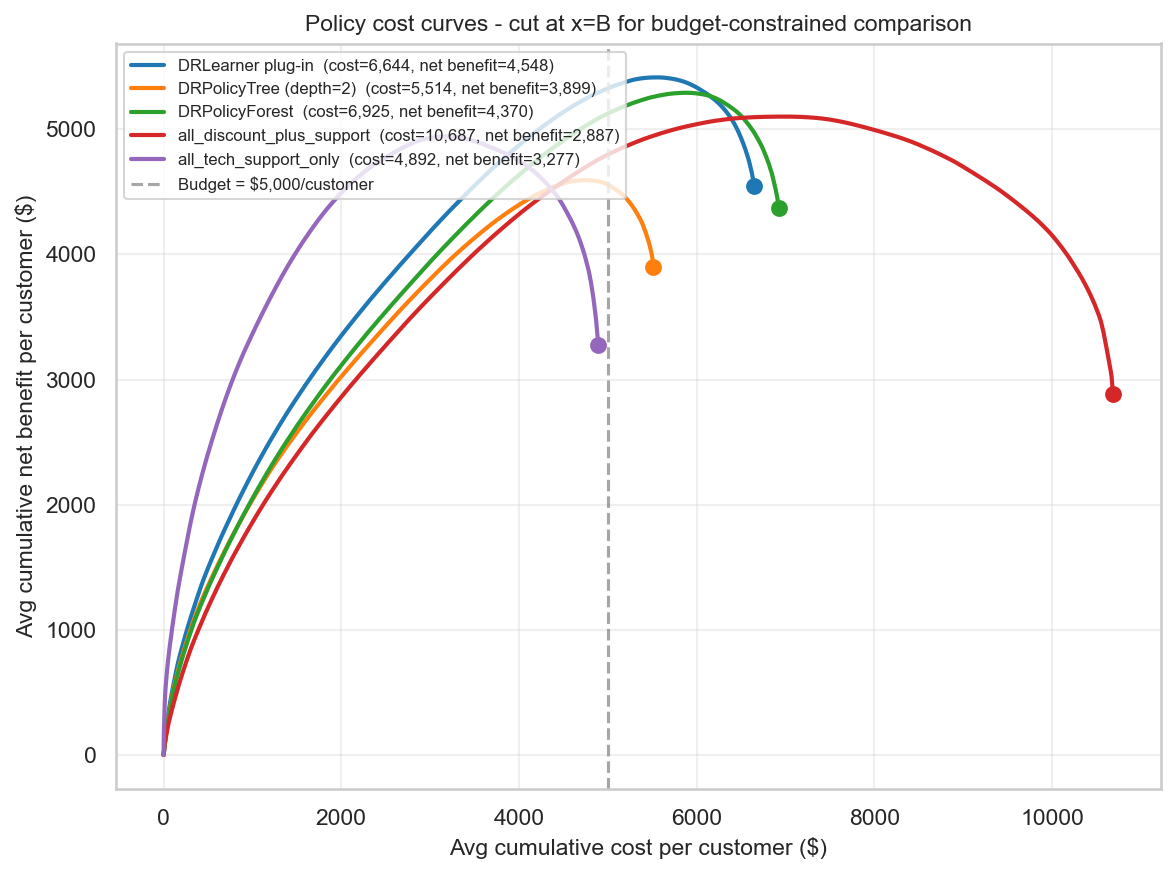
\includegraphics[width=0.78\textwidth]{fig08_cost_curve.png}
\caption{정책별 비용 곡선. 예산($x=B$)에서 y값이 높을수록 효율적이다. 소액 예산에서는 전원 기술지원이, 중간 예산 이상에서는 학습 정책이 앞선다.}
\label{fig:cost}
\end{figure}

\textbf{예산 규모에 따라 효율적인 정책이 다르다.}
\begin{itemize}[leftmargin=1.4em, itemsep=2pt]
  \item \textbf{소액 예산(\$1{,}000\,$\sim$\,3{,}000):} \texttt{all\_tech\_support\_only}가 가장 효율적이다. 기술지원 평균 비용이 낮아 순수익/비용 비율이 높은 고객부터 빠르게 처치할 수 있다.
  \item \textbf{중간 예산(\$4{,}000\,$\sim$\,6{,}000):} 학습 정책(plug-in, forest)이 앞선다. 고객별 최적 처치 배정 효과로 같은 비용에서 더 높은 순이익을 낸다.
  \item \textbf{예산 전부 소진:} 학습 정책이 가장 효율적이다. plug-in은 약 \$6{,}600을 써서 \$4{,}561, forest는 약 \$6{,}900을 써서 \$4{,}376의 순이익을 낸다. 반면 \texttt{all\_discount\_plus\_support}는 \$10{,}700을 전부 소진해도 \$2{,}887에 그쳐 예산 대비 효율이 가장 낮다.
\end{itemize}

\textbf{Q5 요약.} ``어떤 정책이 최선인가''는 예산에 의존한다. 예산이 매우 적으면 저비용 단일 처치가, 예산이 충분하면 타겟팅 정책이 유리하다. 비용 곡선은 예산 의사결정에 직접 활용할 수 있는 도구다.

% =================================================== 결론
\section{결론 및 권고}

약 2{,}000명의 관찰 데이터에서, 비용을 반영한 순이익을 기준으로 네 가지 프로모션의 고객별 최적 배정을 학습했다. 처치 효과의 이질성을 진단(Q1)하고 인과 식별 가정을 점검(Q2)한 뒤, 세 가지 정책을 학습(Q3)하고 학습/평가 데이터를 분리해 doubly robust(AIPW) 기준으로 가치를 비교(Q4)했으며, 예산 제약 하의 효율(Q5)까지 평가했다.

\textbf{비즈니스 권고.}
\begin{enumerate}[leftmargin=1.6em, itemsep=2pt]
  \item \textbf{모두에게 동일한 프로모션을 주지 말고, 타겟팅하라.} 고객별 타겟팅은 최선의 단일 처치 대비 약 12\%, 무처치 대비 약 63\% 높은 순이익을 낸다.
  \item \textbf{배정 기준은 고객 규모와 직원 수다.} 규모가 큰 고객에게는 기술지원+할인, 그 외에는 주로 기술지원을, 기대 순이익이 낮은 일부에게는 무처치를 권한다.
  \item \textbf{예산에 맞춰 정책을 선택하라.} 예산이 빠듯하면 저비용 전원 기술지원이, 1인당 \$4{,}000을 넘어가면 학습 정책으로 전환하는 것이 유리하다.
  \item \textbf{운영 환경에 맞는 모델을 골라라.} 성능 최우선이면 plug-in/forest를, 설명·공정성·운영 안정성이 중요하면 해석 가능한 depth=2 트리 정책을 권한다.
\end{enumerate}

\textbf{한계와 다음 단계.}
\begin{itemize}[leftmargin=1.4em, itemsep=2pt]
  \item 비용은 실제 데이터가 아니라 \textbf{시뮬레이션} 값이다. 실제 비용 데이터가 확보되면 결론이 달라질 수 있다.
  \item Unconfoundedness는 검정 불가능한 가정이다. 가능하다면 소규모 \textbf{무작위 실험(RCT)}으로 학습된 정책을 검증하는 것이 이상적이다.
  \item 표본이 약 1{,}000명(test) 수준이라 정책 간 차이의 신뢰구간이 겹친다. 표본을 늘리면 정책 선택의 확신도가 높아진다.
  \item 다음 단계로 정책 가치의 신뢰구간 추정(부트스트랩), 시간에 따른 정책 모니터링, A/B 테스트 기반 검증을 제안한다.
\end{itemize}

% =================================================== 참고
\section*{\sffamily\color{brand} 참고 자료}
\small
\begin{itemize}[leftmargin=1.4em, itemsep=2pt]
  \item Athey, S., \& Wager, S. (2021). \emph{Policy Learning with Observational Data}. Econometrica. \href{https://arxiv.org/abs/1702.02896}{arxiv.org/abs/1702.02896}
  \item Sun, L., Du, X., Wager, S., et al. (2021). \emph{Treatment Allocation under Uncertain Costs}. \href{https://arxiv.org/abs/2103.11066}{arxiv.org/abs/2103.11066}
  \item Imai, K., \& Li, M. L. (2019). \emph{Experimental Evaluation of Individualized Treatment Rules}. \href{https://arxiv.org/pdf/1905.05389.pdf}{arxiv.org/pdf/1905.05389}
  \item Stanford ML+CI Tutorial --- \emph{Policy Learning I (Binary Treatment)}.
\end{itemize}

\vspace{1em}
{\color{rulegray}\hrule}
\vspace{4pt}
{\footnotesize\color{ink} \textbf{Haechang Cho} · 데이터 분석 포트폴리오 · 코드와 재현 가능한 분석은 GitHub 노트북 참조.}

\end{document}
